%!TEX root =  ssmr_ieee.tex
\section{Performance Evaluation}
\label{sec:evaluation}

%In this section, we describe the environment in which we conducted our experiments, reason about our choice of benchmarks, and experimentally assess Scalable SMR by measuring the performance of the service we implemented on top of Eyrie.

In this section, we assess the performance of Volery with on-disk and in-memory deployments, and local and global commands.
%In this section, we assess the performance of Volery. 
%In Section \ref{sec:environment}, we describe the environment in which we conducted the experiments.
%%, as well as the parameters we used for the client and for the atomic multicast protocol.
%In Sections \ref{sec:disk} and \ref{sec:memory}, we present results for local commands, when Volery is configured with on-disk and in-memory storage, respectively.
%%In Section \ref{sec:memory}, we present the results when storage is done in memory only.
%In Section \ref{sec:global}, we evaluate Volery with global commands.

\subsection{Environment setup and configuration parameters}
\label{sec:environment}

We ran all our experiments on a cluster that had two types of nodes: (a) HP SE1102 nodes, equipped with two Intel Xeon L5420 processors running at 2.5 GHz and with 8 GB of main memory, and (b) Dell SC1435 nodes, equipped with two AMD Opteron 2212 processors running at 2.0 GHz and with 4 GB of main memory. The HP nodes were connected to an HP ProCurve Switch 2910al-48G gigabit network switch, and the Dell nodes were connected to an HP ProCurve 2900-48G gigabit network switch. Those switches were interconnected by a 20 Gbps link. 
%The round-trip latency between nodes connected to different switches was 0.13 ms on average.
All nodes ran CentOS Linux 6.3 with kernel 2.6.32 and had the Oracle Java SE Runtime Environment 7.
% with the \mbox{64-Bit} Server VM (build 24.0-b56).
Before each experiment, we synchronize the clocks of the nodes using NTP.
This is done to obtain accurate values in the measurements of the latency breakdown involving events in different servers.

In all our experiments with Volery and Zookeeper, clients submit commands asynchronously, that is, each client can keep submitting commands even if replies to previous commands have not been received yet, up to a certain number of outstanding commands. 
Trying to issue new commands when this limit is reached makes the client block until some reply is received. 
Replies are processed by callback handlers registered by clients when submitting commands asynchronously. 
We allowed every client to have up to 25 outstanding commands at any time. 
By submitting commands asynchronously, the load on the service can be increased without instantiating new client processes.
%Clients for both Volery and Chirper were implemented this way.
%Zookeeper offers such an asynchronous API, which we used in our experiments. 
Local commands consisted of calls to \verb#setData#, while global commands were invocations to \verb#create# and \verb#delete#. 
``Message size'' and ``command size'', in the next sections, refer to the size of the byte array passed to such commands.
% (except for deletions, which take only a path as parameter).


%We compared Volery with ZKsmr and with Zookeeper.

We compared Volery with the original Zookeeper and with ZKsmr, which is an implementation of the Zookeeper API using traditional state-machine replication. 
For the Zookeeper experiments, we used an ensemble of 3 servers. 
For the other approaches, we used Multi-Ring Paxos for atomic multicast, having 3 acceptors per ring: ZKsmr had 3 replicas that used one Paxos ring to handle all communication, while Volery had 3 replicas per partition, with one Paxos ring per partition, plus one extra ring for commands that accessed multiple partitions. 
Since Zookeeper runs the service and the broadcast protocol (i.e., Zab~\cite{ZAB2011}) in the same machines, each ZKsmr/Volery replica was colocated with a Paxos acceptor in the same node of the cluster. 
We had workloads with three different message sizes: 100, 1000 and 10000 bytes. 
Volery was run with 1, 2, 4 and 8 partitions. 
We conducted all experiments using disk for storage, then using memory (by means of a ramdisk). 
For on-disk experiments, we configured Multi-Ring Paxos with $\Delta$ \cite{MRPPROC2012} of 40 ms, batching timeout of 50 ms and batch size threshold of 250 kilobytes; for in-memory experiments, these parameters were 5 ms, 50 ms and 30 kilobytes, respectively.

%\begin{figure}[ht]
%  \begin{center}
%      \includegraphics[width=\columnwidth]{graphs/results/zk_disk/plot_tp_sizes} 
%    \caption{Normalized throughput versus command size.}
%        \label{fig:zktpdisk}
%  \end{center}
%\end{figure}

\subsection{Experiments using on-disk storage}
\label{sec:disk}

\begin{figure*}

\begin{minipage}[b]{0.5\linewidth} % A minipage that covers half the page
\centering
      \includegraphics[width=0.9\columnwidth]{{graphs/results/zk_disk/plot_tp_lat_multi_0.0readrate}.pdf}
\end{minipage}
\begin{minipage}[b]{0.5\linewidth}
\centering
      \includegraphics[width=0.9\columnwidth]{{graphs/results/zk_disk/timelines_all}.pdf}
\end{minipage}
\caption{Results for Zookeeper, ZKsmr and Volery (with 1, 2, 4 and 8 partitions) using disk. Throughput was normalized by that of Volery with a single partition (absolute values in kilocommands per second are shown). Latencies reported correspond to 75\% of the maximum throughput.}
\label{fig:zkdisk}
\end{figure*}



\begin{figure*}

\begin{minipage}[b]{0.3333\linewidth} % A minipage that covers half the page
\centering
      \includegraphics[width=0.9\columnwidth]{graphs/results/zk_disk/plot_latency_cdfs_100bytes}
\end{minipage}
\begin{minipage}[b]{0.3333\linewidth}
\centering
      \includegraphics[width=0.9\columnwidth]{graphs/results/zk_disk/plot_latency_cdfs_1000bytes}
\end{minipage}
\begin{minipage}[b]{0.3333\linewidth}
\centering
      \includegraphics[width=0.9\columnwidth]{graphs/results/zk_disk/plot_latency_cdfs_10000bytes}
\end{minipage}
\caption{Cumulative distribution function (CDF) of latency for different command sizes (on-disk storage).}
\label{fig:zkdiskcdf}
\end{figure*}



In Figure \ref{fig:zkdisk}, we show results for local commands only.
%Each Paxos acceptor used BerkeleyDB for persistency, where each commit was synchronously written to disk. 
Each Paxos acceptor wrote its vote synchronously to disk before accepting each proposal. 
%Zookeeper was also configured to persist data to disk. 
Zookeeper also persisted data to disk. 
In Figure \ref{fig:zkdisk} (top left), we can see the maximum throughput for each replication scheme and message size, normalized by the throughput of Volery with a single partition. 
In all cases, the throughput of Volery scaled with the number of partitions and, for message sizes of 1000 and 10000 bytes, it scaled linearly (ideal case). 
%
%We can also see that, although Zookeeper had similar or higher throughput than Volery with one partition, having 4 partitions in Volery was enough to make it reach a higher throughput than Zookeeper, in all cases. 
%
For small messages (100 bytes), Zookeeper has similar performance to Volery with a single partition.
As messages increase in size, Zookeeper's throughput improves with respect to Volery: with 1000-byte messages, Zookeeper's throughput is similar to Volery's throughput with two partitions.
For large messages (10000 bytes), Zookeeper is outperformed by Volery with four partitions.
%
Comparing S-SMR with traditional SMR, we can see that for small messages (100 bytes), ZKsmr performed better than Volery with one partition. 
This is due to the additional complexity added by Eyrie in order to ensure linearizability when data is partitioned. 
Such difference in throughput is less significant with bigger commands (1000 and 10000 bytes).

We can also see in Figure \ref{fig:zkdisk} (bottom left), the latency values for the different implementations tested. 
Latency values correspond to 75\% of the maximum throughput.
Zookeeper has the lowest latency for 100- and 1000-byte command sizes. 
For 10000-byte commands, Volery had similar or lower latency than Zookeeper. 
Such lower latency of Volery with 10000-byte commands is due to a shorter time spent with batching: as message sizes increase, the size threshold of the batch (250 kilobytes for on-disk storage) is reached faster, resulting in lower latency. %Evidence for this phenomenon is given in Figure \ref{fig:zkdisk} (right).

Figure \ref{fig:zkdisk} (right) shows the latency breakdown of commands executed by Volery.
% down into its components, showing how much time is spent in each phase of the command's path between the client sending the command until the end of the command's execution. 
\emph{Batching} is the time elapsed from the moment the client sends command $C$ to the instant when $C$ is proposed by the ring coordinator as part of a batch. 
\emph{Multicasting} is the time between the propose is executed until the batch that contains $C$ is delivered by a server replica. 
\emph{Waiting} represents the time between the delivery and the moment when $C$ finally starts executing.
\emph{Executing} measures the delay between the start of the execution of command $C$ until the client receives $C$'s response.
We can see that more than half of the latency time is due to multicasting, which includes saving Multi-Ring Paxos instances synchronously to disk. 
There is also a significant amount of time spent with batching, done to reduce the number of disk operations and allow higher throughput: each Paxos proposal is saved to disk synchronously, so increasing the number of commands per proposal (i.e., per batch) reduces the number of times the disk is accessed.
%This allows performance to increase, but comes at the cost of increased latency.
This allows performance to improve, but increases latency.

%Having a more complex implementation, which took partitioning into account, made Volery have a higher average latency than ZKsmr and Zookeeper. As the message size increased, all approaches had higher latency, although there did not seem to exist a correlation of increased latencies as the number of partitions increased, in these experiments.

In Figure \ref{fig:zkdiskcdf}, we show the cumulative distribution functions (CDFs) of latency for all experiments where disk was used for storage. 
The results show that the latency distributions for ZKsmr and Volery with a single partition are similar, while latency had more variation for 2, 4 and 8 partitions. 
An important difference between deployments with a single and with multiple partitions is related to how Multi-Ring Paxos is used. In ZKsmr and in Volery with a single partition, there is only one Paxos ring, which orders all commands from all clients and delivers them to all replicas. 
When there are multiple partitions, each replica delivers messages from two rings: one ring that orders messages related to the replica's partition only, and another ring that orders messages addressed to more than one partition---each replica deterministically merges deliveries from multiple rings. 
As the time necessary to perform such deterministic merge is influenced by the level of synchrony of the rings, latency is expected to fluctuate more when merging is involved.

\subsection{Experiments using in-memory storage}
\label{sec:memory}

\begin{figure*}

\begin{minipage}[b]{0.5\linewidth} % A minipage that covers half the page
\centering
      \includegraphics[width=0.9\columnwidth]{{graphs/results/zk_mem/plot_tp_lat_multi_0.0readrate}.pdf}
\end{minipage}
\begin{minipage}[b]{0.5\linewidth}
\centering
      \includegraphics[width=0.9\columnwidth]{{graphs/results/zk_mem/timelines_all}.pdf}
\end{minipage}
\caption{Results for Zookeeper, ZKsmr and Volery (with 1, 2, 4 and 8 partitions) using memory. Throughput was normalized by that of Volery with a single partition (absolute values in kilocommands per second are shown). Latencies reported correspond to 75\% of the maximum throughput.}
\label{fig:zkmem}

\end{figure*}



\begin{figure*}

\begin{minipage}[b]{0.3333\linewidth} % A minipage that covers half the page
\centering
      \includegraphics[width=0.9\columnwidth]{graphs/results/zk_mem/plot_latency_cdfs_100bytes}
\end{minipage}
\begin{minipage}[b]{0.3333\linewidth}
\centering
      \includegraphics[width=0.9\columnwidth]{graphs/results/zk_mem/plot_latency_cdfs_1000bytes}
\end{minipage}
\begin{minipage}[b]{0.3333\linewidth}
\centering
      \includegraphics[width=0.9\columnwidth]{graphs/results/zk_mem/plot_latency_cdfs_10000bytes}
\end{minipage}
\caption{Cumulative distribution function (CDF) of latency for different command sizes (in-memory storage).}
\label{fig:zkmemcdf}
\end{figure*}

In Figure \ref{fig:zkmem}, we show the results for local commands when storing data in memory only. 
Volery's throughput scales with the number of partitions (Figure \ref{fig:zkmem} (top left)), specially for large messages, in which case the scalability is linear with the number of partitions (i.e., ideal case). 
We can also see that latency values for Volery and ZKsmr are less than half of what they are for on-disk storage (Figure \ref{fig:zkmem} (bottom left)), while Zookeeper's latency decreased by an order of magnitude. 
%The difference in latency is due to the atomic multicast library (URingPaxos) we use, while Zookeeper uses Zab, which is a greatly optimised atomic broadcast algorithm.
These results suggest that further improvements should be achievable in the in-memory Volery configuration with additional optimizations and finer tuning of the atomic multicast parameters.

Figure \ref{fig:zkmem} (right) shows the latency breakdown. 
Even though no data is saved to disk, multicasting is still responsible for most of the latency, followed by batching. 
Differently from the experiments described in Section \ref{sec:disk}, batching here had a size threshold of 30 kilobytes, which helps to explain why batching time is roughly the same for different message sizes. 
In these experiments, although there are no disk writes, batching is still used because it reduces the number of Paxos proposals and the number of messages sent through the network, which allows higher throughput. 
Figure~\ref{fig:zkmemcdf} shows the latency CDFs for the in-memory experiments, where we can see that Volery with multiple partitions (i.e., deployments where Multi-Ring Paxos uses multiple rings) tends to have more variation in latency.

\subsection{Experiments with global commands}
\label{sec:global}

In this section, we analyze how Volery performs when the workload includes commands that are multicast to all partitions (global commands). This is the least favorable (non-faulty) scenario for S-SMR, as having commands multicast to all partitions effectively reduces scalability: if all commands go to all partitions, adding more partitions will not increase throughput.

We ran experiments with different rates of global commands (i.e., create and delete operations): 0\%, 1\%, 5\% and 10\% of all commands. 
We chose such rates for two reasons: (i) it is obvious that high rates of global commands will prevent the system from scaling, plus (ii) it is common for large scale services to have a high rate of read requests (which are local commands in Volery). 
An example of such a service is Facebook's TAO~\cite{facebookTAO}, which handles requests to a social graph; it allows, for instance, pages to be generated based on the user's connections in the social network. 
In Facebook's TAO, 99.8\% of all requests are read-only~\cite{facebookTAO}. 
%With this kind of workload in mind, 10\% is a \emph{very} high rate of global commands.

\begin{figure*}

\begin{minipage}[b]{0.5\linewidth} % A minipage that covers half the page
\centering
      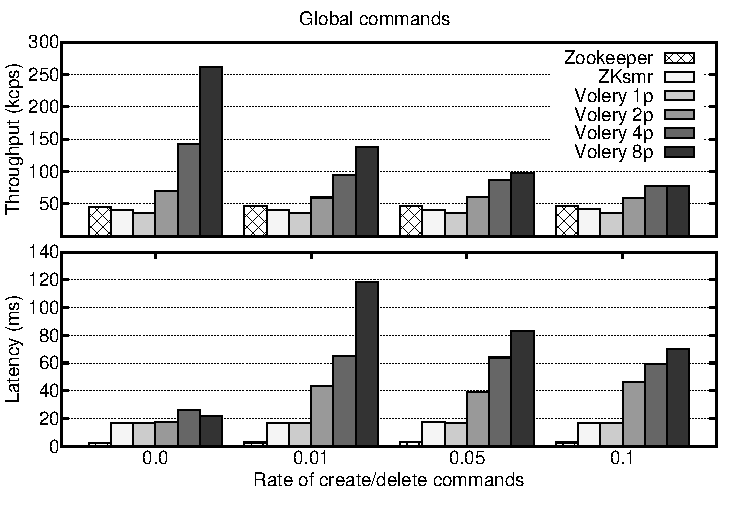
\includegraphics[width=0.9\columnwidth]{{graphs/results/zk_multipartition/plot_tp_lat_multi_global}.pdf}
\end{minipage}
\begin{minipage}[b]{0.5\linewidth}
\centering
      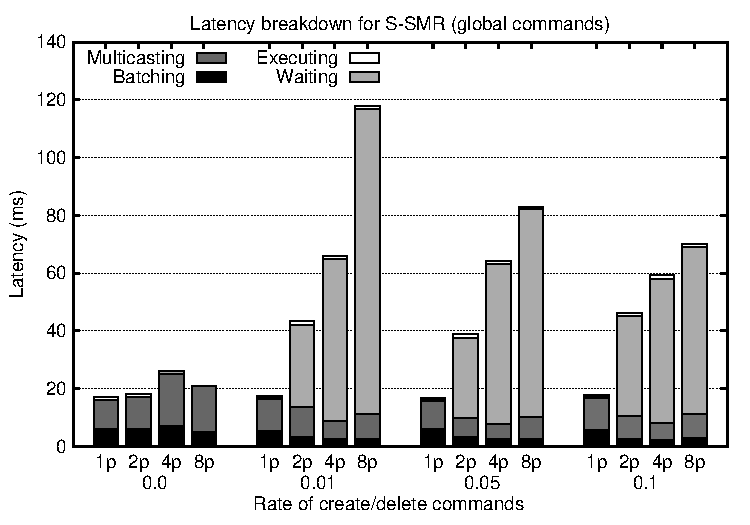
\includegraphics[width=0.9\columnwidth]{{graphs/results/zk_multipartition/timelines_global}.pdf}
\end{minipage}
\caption{Throughput and latency versus rate of create/delete commands (in-memory storage, 1000-bytes commands). Throughput is shown in units of a thousand commands per second (kcps). Latencies shown corresponds to 75\% of the maximum throughput.}
\label{fig:zkglobal}
\end{figure*}

\begin{figure*}

\begin{minipage}[b]{0.3333\linewidth} % A minipage that covers half the page
\centering
      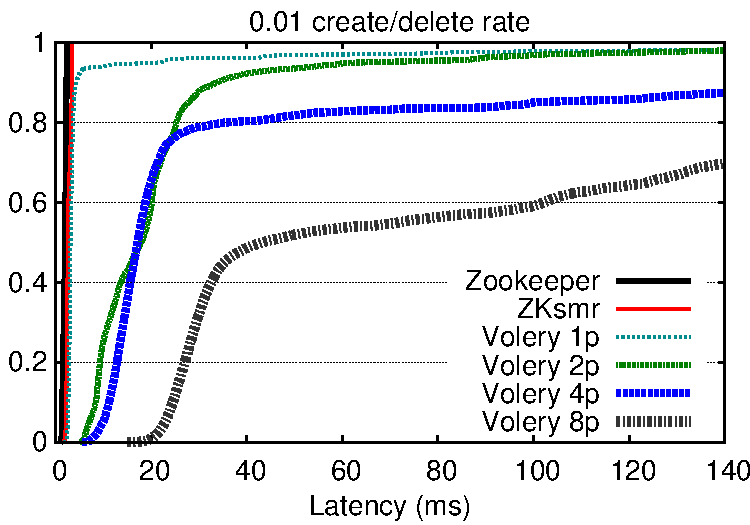
\includegraphics[width=0.9\columnwidth]{{graphs/results/zk_multipartition/plot_latency_cdfs_globalrate_0.01}.pdf}
\end{minipage}
\begin{minipage}[b]{0.3333\linewidth}
\centering
      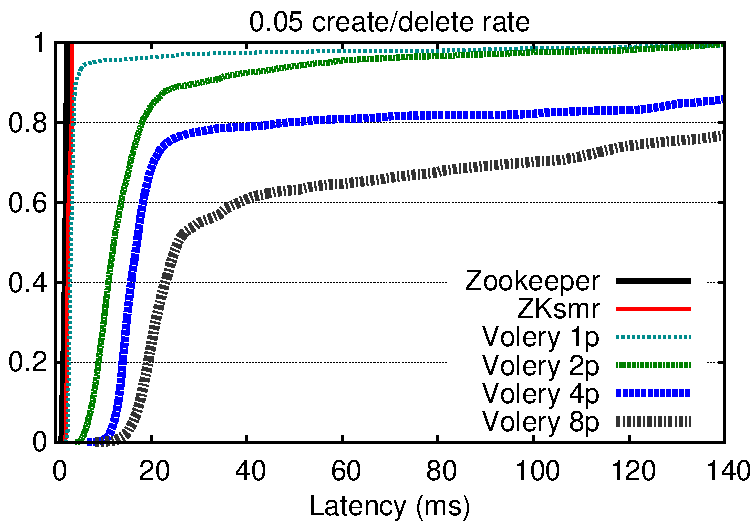
\includegraphics[width=0.9\columnwidth]{{graphs/results/zk_multipartition/plot_latency_cdfs_globalrate_0.05}.pdf}
\end{minipage}
\begin{minipage}[b]{0.3333\linewidth}
\centering
      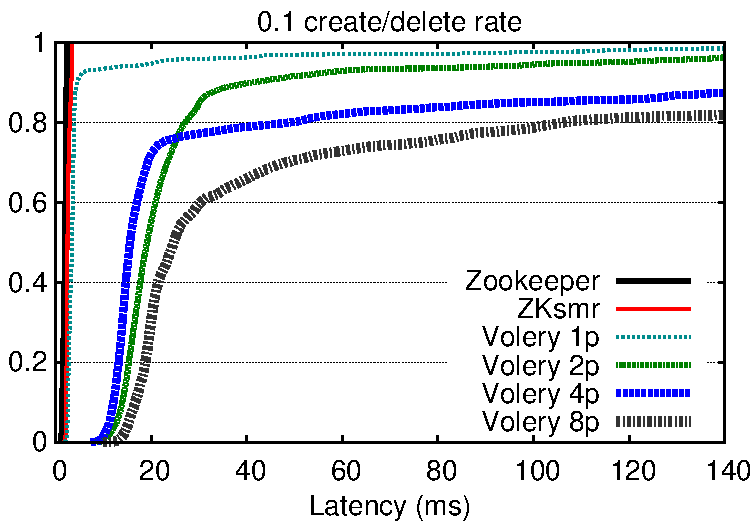
\includegraphics[width=0.9\columnwidth]{{graphs/results/zk_multipartition/plot_latency_cdfs_globalrate_0.1}.pdf}
\end{minipage}
\caption{Cumulative distribution function (CDF) of latency for different rates of create/delete commands (in-memory storage, 1000-bytes commands).}
\label{fig:zkglobalcdf}
\end{figure*}



We can see in Figure \ref{fig:zkglobal} (top left) that Volery scales throughput with the number of partitions for all configurations but the exceptional case of 10\% of global commands when augmenting the number of partitions from 4 to 8.
Moreover, Volery with two partitions outperforms the Zookeeper in all experiments.
The major drawback of Volery under global commands is that to ensure linearizability, partitions must exchange signals: as \verb#create# and \verb#delete# commands are multicast to all partitions, no server can send a reply to a client before receiving a signal from \emph{all} other partitions when executing such a command. 
This explains the significant increase in latency shown in Figure \ref{fig:zkglobal} (bottom left), as global commands are added to the workload: as the number of partitions increases, so does the average latency. 
As we can see in Figure \ref{fig:zkglobal} (right), this extra latency comes from the servers waiting for signals from other partitions.

Figure \ref{fig:zkglobalcdf} shows the latency CDFs for the workloads with global commands. 
For experiments with more than one partition, the rate of messages with high latency is much higher than the rate of global commands. 
This happens due to a ``convoy effect": local commands may be delivered after global commands, having to wait for the latter to finish.
%This happens due to a ``convoy effect": local commands may be delivered after global commands and, therefore, must wait for the latter to finish executing.%, which delays the execution of the local commands.

%\subsection{Chirper experiments}
%
%TODO: every request touching x partitions; 1 experiment for each x in \{1, 2, 4, 8\}, when the system has p partitions, with p in \{1, 2, 4, 8\}
%
%We have also simulated a social network using detailed statistics of real Twitter usage, which can be found online.\footnote{http://www.sysomos.com/insidetwitter/} In such experiment, we simulated 100,000 users. Each user followed $f$ friends, where such friends were divided among $p$ partitions. The resulting graph was made so that each user would have $r$ followers. For each user, we decide values $f$, $p$ and $r$ randomly, based on the statistics we have found: we made both $f$ and $r$ follow a Zipfian distribution with size 100 and skew 1, while $p$ followed a Zipfian distribution with size $P$ (total number of partitions in the system) and skew 1. Also, according to the statistics we have used, 5\% of all Twitter users were responsible for 75\% of all Twitter activity (i.e., number of tweets), while 10\% were responsible for 86\% of all activity, and so on, approximately fitting a Zipfian distribution with size 100 and skew 1.6, where the most active users were the ones with most followers, so our simulated social network also had this characteristic. We used the same distribution for timeline requests, having the users with most friends (i.e., those who follow the most people) requesting their timeline more frequently than other users.